\section{پیش‌زمینه}
در بحث‌های قبلی اجرای کوئری‌ها فرض بر این بود که کوئری‌ها با یک worker (یعنی thread) اجرا می‌شوند. با این حال، در عمل، کوئری‌ها اغلب به صورت موازی با چندین worker اجرا می‌شوند.
اجرای موازی مزایای کلیدی متعددی برای DBMS ها فراهم می‌کند:
\begin{itemize}
	\item افزایش عملکرد در میزان گذردهی (تعداد بیشتر کوئری‌ها در ثانیه) و زمان پاسخ‌دهی (زمان کمتر برای هر کوئری).
	
	\item افزایش پاسخگویی و دسترس‌پذیری از دید مشتریان خارجی DBMS.
	
	\item کاهش کل هزینه مالکیت. این هزینه شامل هم خرید سخت‌افزار و لایسنس نرم‌افزار، و هم سربار نیروی انسانی برای پیاده‌سازی DBMS و انرژی مورد نیاز برای اجرای ماشین‌ها می‌شود.
\end{itemize}
دو نوع موازی‌سازی وجود دارد که DBMSها پشتیبانی می‌کنند: \lr{inter-query parallelism} و \lr{intra-query parallelism}.

\section{پایگاه‌داده‌های Parallel در مقابل Distributed}
در هر دو سیستم موازی و توزیع‌شده، پایگاه‌داده در میان چندین "منبع" پراکنده شده است تا موازی‌سازی بهبود یابد. این منابع ممکن است محاسباتی (مثل هسته‌های CPU، سوکت‌های CPU، GPUها، ماشین‌های اضافی) یا ذخیره‌سازی (مثل دیسک‌ها، حافظه) باشند.
تمایز بین سیستم‌های موازی و توزیع‌شده مهم است:
\begin{itemize}
	\item \textbf{پایگاه‌داده موازی (Parallel-DBMS)}: در یک پایگاه‌داده موازی، منابع یا گره‌ها از لحاظ فیزیکی به هم نزدیک هستند. این گره‌ها از طریق یک اتصال سریع (high-speed-interconnect) با یکدیگر ارتباط برقرار می‌کنند. فرض بر این است که ارتباط بین منابع نه تنها سریع، بلکه ارزان و قابل اطمینان است.
	
	\item \textbf{پایگاه‌داده توزیع‌شده (Distributed-DBMS)}: در یک پایگاه‌داده توزیع‌شده، منابع ممکن است از هم دور باشند؛ این ممکن است به معنای پراکندگی پایگاه‌داده در قفسه‌ها یا مراکز داده در نقاط مختلف جهان باشد. در نتیجه، منابع از طریق یک اتصال کندتر (اغلب از طریق یک شبکه عمومی) ارتباط برقرار می‌کنند. هزینه‌های ارتباط بین گره‌ها بیشتر است و نمی‌توان از خرابی‌ها چشم‌پوشی کرد.
\end{itemize}
حتی اگر پایگاه‌داده به طور فیزیکی بر روی چندین منبع تقسیم شده باشد، هنوز به صورت یک نمونه پایگاه‌داده منطقی واحد برای برنامه ظاهر می‌شود. بنابراین، یک کوئری SQL که در برابر یک پایگاه‌داده تک‌گره‌ای اجرا می‌شود باید نتیجه یکسانی در یک پایگاه‌داده موازی یا توزیع‌شده تولید کند.


\section{مدل‌های فرآیند}
یک مدل فرآیند DBMS تعیین می‌کند که سیستم چگونه از درخواست‌های همزمان از یک برنامه/محیط چندکاربره پشتیبانی می‌کند. DBMS شامل یک یا چند worker است که مسئول اجرای وظایف به نمایندگی از مشتری و بازگرداندن نتایج هستند. یک برنامه ممکن است یک درخواست بزرگ یا چندین درخواست را به طور همزمان ارسال کند که باید بین workerهای مختلف تقسیم شود.

\qquad\qquad\qquad	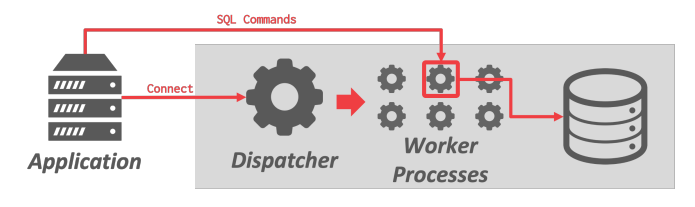
\includegraphics[width=0.7\linewidth]{screenshot009}

دو مدل فرآیند اصلی وجود دارد که یک DBMS ممکن است اتخاذ کند: فرآیند به ازای worker و thread به ازای worker. یک الگوی استفاده رایج دیگر از پایگاه‌داده رویکرد تعبیه شده را اتخاذ می‌کند.

\subsection{Process-per-Worker}
پایه‌ای‌ترین رویکرد، فرآیند به ازای worker است. در اینجا، هر worker یک فرآیند جداگانه سیستم‌عامل است و بنابراین به برنامه‌ریز (scheduler) سیستم‌عامل متکی است. یک برنامه درخواست ارسال می‌کند و یک اتصال به سیستم پایگاه‌داده باز می‌کند. یک توزیع‌کننده (dispatcher) درخواست را دریافت می‌کند و یکی از فرآیندهای worker خود را برای مدیریت اتصال انتخاب می‌کند. برنامه سپس مستقیماً با workerی که مسئول اجرای درخواستی است که کوئری می‌خواهد، ارتباط برقرار می‌کند. این توالی از رویدادها در شکل ۱ نشان داده شده است.

اتکا به سیستم‌عامل برای برنامه‌ریزی به طور موثر کنترل DBMS بر اجرای کارها را کاهش می‌دهد. علاوه بر این، این مدل برای نگهداری ساختارهای داده جهانی به حافظه مشترک متکی است یا به پیام‌رسانی متکی است که سربار بیشتری دارد.

یکی از مزایای رویکرد فرآیند به ازای worker این است که خرابی یک فرآیند کل سیستم را مختل نمی‌کند زیرا هر worker در زمینه فرآیند سیستم‌عامل خود اجرا می‌شود.

این مدل فرآیند مساله کارگران متعدد در فرآیندهای جداگانه که نسخه‌های متعددی از همان صفحه را می‌سازند، ایجاد می‌کند. یک راه‌حل برای به حداکثر رساندن استفاده از حافظه، استفاده از حافظه مشترک برای ساختارهای داده جهانی است تا بتوانند توسط کارگرانی که در فرآیندهای مختلف اجرا می‌شوند، به اشتراک گذاشته شوند.

نمونه‌هایی از سیستم‌هایی که از مدل فرآیند به ازای worker استفاده می‌کنند شامل Postgres و Oracle هستند. زمانی که این DBMSها توسعه یافتند، pthreads هنوز به استاندارد مدل threading تبدیل نشده بود. معنای threading از یک سیستم‌عامل به سیستم‌عامل دیگر متفاوت بود در حالی که \texttt{fork()} بهتر تعریف شده بود.

\subsection{Thread-per-Worker}
مدل رایج امروزی thread به ازای worker است. به جای داشتن فرآیندهای مختلف برای انجام وظایف مختلف، هر سیستم پایگاه‌داده فقط یک فرآیند با چندین thread worker دارد. در این محیط، DBMS کنترل کامل بر وظایف و thread ها دارد و می‌تواند برنامه‌ریزی خود را مدیریت کند. مدل چند thread ممکن است از یک thread توزیع‌کننده استفاده کند یا نکند.

استفاده از معماری چند thread مزایای خاصی فراهم می‌کند. اولاً، سربار کمتری برای هر تعویض زمینه (context switch) وجود دارد. علاوه بر این، نیازی به نگهداری مدل مشترک نیست. با این حال، ممکن است که خرابی یک thread کل فرآیند پایگاه‌داده را از کار بیاندازد. همچنین، مدل thread به ازای worker لزوماً به این معنا نیست که DBMS از موازی‌سازی درون کوئری 
(intra-query-parallelism) پشتیبانی می‌کند.

تقریباً هر DBMS ایجاد شده در ۲۰ سال گذشته از این رویکرد استفاده می‌کند، از جمله SQL Server  و MySQL و Oracle مدل‌های خود را به‌روزرسانی کرده‌اند تا از این رویکرد پشتیبانی کنند. Postgres و پایگاه‌داده‌های مشتق شده از Postgres عمدتاً هنوز از رویکرد مبتنی بر فرآیند استفاده می‌کنند.

\pagebreak

\qquad\qquad\qquad	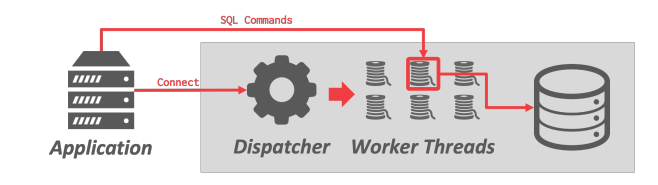
\includegraphics[width=0.7\linewidth]{screenshot011}

\qquad\qquad\qquad	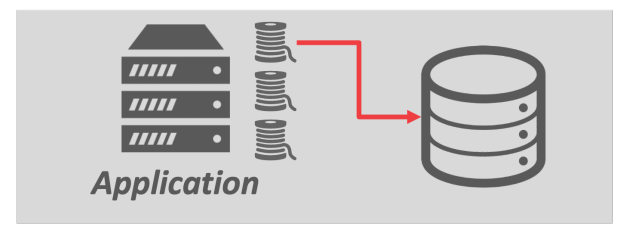
\includegraphics[width=0.7\linewidth]{screenshot012}

\subsection{زمان‌بندی}
در نتیجه، برای هر برنامه کوئری، DBMS باید تصمیم بگیرد کجا، چه زمانی و چگونه اجرا کند. سوالات مرتبط شامل موارد زیر هستند:
\begin{itemize}
	\item از چند وظیفه باید استفاده کند؟
	\item از چند هسته CPU باید استفاده کند؟
	\item وظایف باید روی کدام هسته‌های CPU اجرا شوند؟
	\item خروجی وظیفه باید کجا ذخیره شود؟
\end{itemize}
هنگام تصمیم‌گیری در مورد برنامه‌های کوئری، DBMS همیشه بیشتر از سیستم‌عامل می‌داند و باید به همین ترتیب اولویت داده شود.

\subsection{Embedded-DBMS}
یک الگوی استفاده بسیار متفاوت برای پایگاه‌داده‌ها شامل اجرای سیستم در همان فضای آدرس برنامه است، برخلاف مدل مشتری-سرور که در آن پایگاه‌داده مستقل از برنامه است. در این سناریو، برنامه وظایف و threadها را برای اجرا روی سیستم پایگاه‌داده تنظیم می‌کند. خود برنامه تا حد زیادی مسئول زمان‌بندی خواهد بود. نموداری از رفتارهای زمان‌بندی یک DBMS تعبیه‌شده در شکل ۳ نشان داده شده است.

DuckDB، SQLite و RocksDB مشهورترین DBMSهای تعبیه‌شده هستند.

\pagebreak

\section{موازی‌سازی بین کوئری‌ها (Inter-Query-Parallelism)}
در موازی‌سازی بین کوئری‌ها، DBMS کوئری‌های مختلف را به طور همزمان اجرا می‌کند. از آنجا که چندین worker به صورت همزمان درخواست‌ها را اجرا می‌کنند، عملکرد کلی بهبود می‌یابد. این امر گذردهی را افزایش داده و زمان تاخیر را کاهش می‌دهد.

اگر کوئری‌ها فقط خواندنی باشند، هماهنگی کمی بین کوئری‌ها مورد نیاز است. با این حال، اگر چندین کوئری به طور همزمان در حال به‌روزرسانی پایگاه‌داده باشند، تعارضات پیچیده‌تری ایجاد می‌شود.

\qquad\qquad\qquad	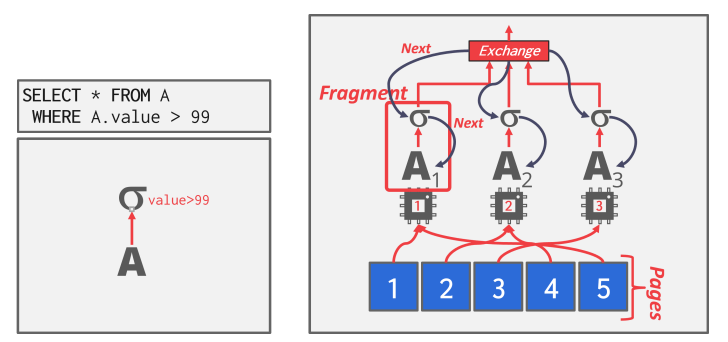
\includegraphics[width=0.7\linewidth]{screenshot013}

برنامه کوئری برای این SELECT یک اسکن ترتیبی روی A است که به یک عملگر فیلتر تغذیه می‌شود. برای اجرای این به صورت موازی، برنامه کوئری به بخش‌های مجزا تقسیم می‌شود. یک بخش برنامه مشخص توسط یک worker متمایز اجرا می‌شود. عملگر تبادل (exchange-operator) به طور همزمان \texttt{Next} را روی همه بخش‌ها فراخوانی می‌کند که سپس داده‌ها را از صفحات مربوطه خود بازیابی می‌کنند.

\section{موازی‌سازی درون کوئری (Intra-Query-Parallelism)}
در موازی‌سازی درون کوئری، DBMS عملیات یک کوئری واحد را به صورت موازی اجرا می‌کند. این امر زمان تاخیر کوئری‌های طولانی‌مدت را کاهش می‌دهد.

سازماندهی موازی‌سازی درون کوئری را می‌توان از دیدگاه پارادایم تولیدکننده/مصرف‌کننده در نظر گرفت. هر عملگر تولیدکننده داده‌ها و همچنین مصرف‌کننده داده‌ها از یک عملگر دیگر که در زیر آن اجرا می‌شود، است. الگوریتم‌های موازی برای هر عملگر رابطه‌ای وجود دارد. DBMS می‌تواند از چندین thread برای دسترسی به ساختارهای داده متمرکز استفاده کند یا از تقسیم‌بندی برای تقسیم کار استفاده کند.

درون موازی‌سازی درون کوئری، سه نوع موازی‌سازی وجود دارد: درون‌عملگر، بین‌عملگر، و بوشی (bushy). این روش‌ها متقابلاً انحصاری نیستند. مسئولیت DBMS این است که این تکنیک‌ها را به گونه‌ای ترکیب کند که عملکرد را بر روی بار کاری داده شده بهینه کند.

\subsubsection{موازی‌سازی درون‌عملگر (افقی)}
در موازی‌سازی درون‌عملگر، عملگرهای برنامه کوئری به بخش‌های مستقل تجزیه می‌شوند که همان عملکرد را بر روی زیرمجموعه‌های متفاوت (مجزا) از داده‌ها انجام می‌دهند.

DBMS یک عملگر تبادل (exchange operator) را در برنامه کوئری درج می‌کند تا نتایج را از عملگرهای فرزند جمع کند. عملگر تبادل از اجرای عملگرهای بالاتر در برنامه تا زمانی که تمام داده‌ها را از فرزندان دریافت کند، جلوگیری می‌کند. نمونه‌ای از این در شکل ۴ نشان داده شده است.
\pagebreak

به طور کلی، سه نوع عملگر تبادل وجود دارد:
\begin{itemize}
	\item \textbf{Gather}: ترکیب نتایج از چندین worker به یک جریان خروجی واحد. این نوع رایج‌ترین نوع مورد استفاده در DBMSهای موازی است.
	\item \textbf{Distribute}: تقسیم یک جریان ورودی به چندین جریان خروجی.
	\item \textbf{Repartition}: سازماندهی مجدد چندین جریان ورودی در چندین جریان خروجی. این امکان را به DBMS می‌دهد که ورودی‌هایی که به یک روش تقسیم شده‌اند را گرفته و سپس به روش دیگری توزیع کند.
\end{itemize}


\subsubsection{موازی‌سازی بین‌عملگر (عمودی)}
در موازی‌سازی بین‌عملگر، DBMS عملگرها را به گونه‌ای همپوشانی می‌کند که داده‌ها را از یک مرحله به مرحله بعدی بدون ماده‌سازی انتقال دهد. این گاهی اوقات به عنوان موازی‌سازی لوله‌ای (pipelined-parallelism) نامیده می‌شود.

\qquad\qquad\qquad	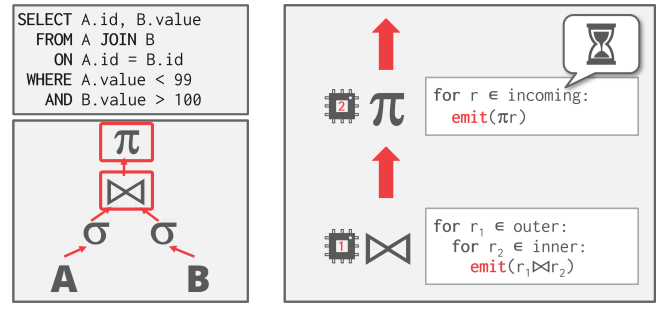
\includegraphics[width=0.7\linewidth]{screenshot014}


در عبارت JOIN سمت چپ، یک worker عملیات join را انجام می‌دهد و سپس نتیجه را به worker دیگری ارسال می‌کند که عملیات projection را انجام می‌دهد و سپس نتیجه را دوباره ارسال می‌کند.

\qquad\qquad\qquad	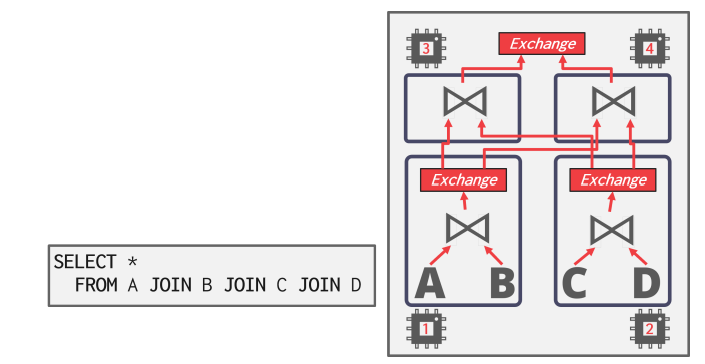
\includegraphics[width=0.7\linewidth]{screenshot015}

برای انجام یک JOIN چهارطرفه روی سه جدول، برنامه کوئری به چهار بخش تقسیم می‌شود همان‌طور که نشان داده شده است. بخش‌های مختلف برنامه کوئری به طور همزمان اجرا می‌شوند، به روشی مشابه با موازی‌سازی بین‌عملگر.
این رویکرد به طور گسترده در سیستم‌های پردازش جریان استفاده می‌شود، که سیستم‌هایی هستند که به طور مداوم یک کوئری را بر روی جریان ورودی tupleها اجرا می‌کنند.

\subsubsection{موازی‌سازی بوشی (Bushy-Parallelism)}
موازی‌سازی بوشی یک ترکیب از موازی‌سازی درون‌عملگر و بین‌عملگر است که در آن worker ها عملگرهای متعدد از بخش‌های مختلف برنامه کوئری را به طور همزمان اجرا می‌کنند.
DBMS همچنان از عملگرهای تبادل برای ترکیب نتایج میانی از این بخش‌ها استفاده می‌کند.


\section{موازی‌سازی I/O}
استفاده از thread اضافی برای اجرای کوئری‌ها به صورت موازی عملکرد را بهبود نمی‌بخشد اگر دیسک همیشه گلوگاه اصلی باشد. بنابراین، مهم است که بتوان پایگاه‌داده را در چندین دستگاه ذخیره‌سازی تقسیم کرد.

برای رفع این مشکل، DBMS ها از موازی‌سازی I/O برای تقسیم نصب بر روی چندین دستگاه استفاده می‌کنند. دو رویکرد برای موازی‌سازی I/O وجود دارد: 
\begin{enumerate}
	\item موازی‌سازی چند دیسک
	\item پارتیشن‌بندی پایگاه‌داده
\end{enumerate}

\subsection{موازی‌سازی چند دیسک}
در موازی‌سازی چند دیسک، سیستم‌عامل/سخت‌افزار برای ذخیره فایل‌های DBMS در چندین دستگاه ذخیره‌سازی پیکربندی می‌شود. این می‌تواند از طریق دستگاه‌های ذخیره‌سازی یا پیکربندی RAID انجام شود. تمام تنظیمات ذخیره‌سازی برای DBMS شفاف است، بنابراین workerها نمی‌توانند بر روی دستگاه‌های مختلف عمل کنند زیرا DBMS از موازی‌سازی زیرساختی آگاه نیست.

\subsection{پارتیشن‌بندی پایگاه‌داده}
در پارتیشن‌بندی پایگاه‌داده، پایگاه‌داده به زیرمجموعه‌های مجزا تقسیم می‌شود که می‌توانند به دیسک‌های مجزا اختصاص داده شوند. برخی از DBMS ها اجازه مشخص کردن مکان دیسک هر پایگاه‌داده فردی را می‌دهند. این کار در سطح سیستم‌فایل آسان است اگر DBMS هر پایگاه‌داده را در یک دایرکتوری جداگانه ذخیره کند. فایل لاگ تغییرات معمولاً به اشتراک گذاشته می‌شود.

ایده پارتیشن‌بندی منطقی این است که یک جدول منطقی واحد به بخش‌های فیزیکی مجزا تقسیم شود که به صورت جداگانه ذخیره/مدیریت می‌شوند. چنین پارتیشن‌بندی به طور ایده‌آل برای برنامه شفاف است. یعنی برنامه باید بتواند به جداول منطقی دسترسی پیدا کند بدون اینکه نگران چگونگی ذخیره‌سازی باشد.

ما این رویکردها را در ادامه ترم و در زمان بحث درباره پایگاه‌داده‌های توزیع‌شده پوشش خواهیم داد.






